\documentclass[graphics, twocolumn, usenatbib]{mn2e}
\usepackage[utf8]{inputenc}
\usepackage{times}
\usepackage{natbib} 
\usepackage{epsfig} 
\usepackage{graphicx} 
\usepackage{color}
%\usepackage{deluxetable} 
\usepackage{aas_macros} 
\usepackage{amssymb}
\usepackage{amsmath}
\usepackage[title]{appendix}
\usepackage{hyperref}	% Hyperlinks
\hypersetup{colorlinks=true,linkcolor=blue,citecolor=blue,filecolor=blue,urlcolor=blue}
\usepackage[caption=false]{subfig}
\newcommand{\lya}{Lyman-$\alpha$~}
\newcommand{\gad}{\textsc{Gadget-2~}}
\newcommand{\enzo}{\texttt{Enzo~}}
\newcommand{\yt}{\texttt{yt}}
\newcommand{\enzoc}{\texttt{Enzo}}
\newcommand{\grackle}{\texttt{Grackle-2.1~}}
\newcommand{\gracklec}{\texttt{Grackle-2.1}}
\newcommand{\enzolat}{\texttt{Enzo-2.3}}
\newcommand{\cosmos}{\textsc{Cosmos~}}
\newcommand{\darwin}{\textsc{Darwin~}}
\newcommand{\enzoamr}{\texttt{Enzo(AMR)~}}
\newcommand{\enzost}{\texttt{Enzo(static)~}}
\newcommand{\lyb}{Lyman-$\beta$~} 
\newcommand{\eg}{{\it e.g.~}}
\newcommand{\kms} {km $\rm{s^{-1}}$}
\newcommand{\mpch} {\rm $h^{-1}$ Mpc\,\,} 
\newcommand{\kpch} {\rm $h^{-1}$ kpc\,\,} 
\newcommand{\msolar} {$\rm{M_{\odot}}~$}
\newcommand{\msolarc} {$\rm{M_{\odot}}$}
\newcommand{\msolaryr} {$\rm{M_{\odot}/yr}~$}
\newcommand{\msolaryrc} {$\rm{M_{\odot}/yr}$}
\newcommand{\lsolar} {$\rm{L_{\odot}}~$}
\newcommand{\lsolarc} {$\rm{L_{\odot}}$}
\newcommand{\zsolar} {$\rm{Z_{\odot}}~$}
\newcommand{\zsolarc} {$\rm{Z_{\odot}}$}
\newcommand{\rsolar} {$\rm{R_{\odot}}~$}
\newcommand{\molH} {$\rm{H_2}$~}
\newcommand{\molHc} {$\rm{H_2}$}
\newcommand{\J} {$\rm{10^{-21}\ erg\ cm^{-2}\ s^{-1}\ Hz^{-1}\ sr^{-1}}$}
\newcommand{\inten} {$\rm{ erg\ cm^{-2}\ s^{-1}\ Hz^{-1}\ sr^{-1}}$~}
\newcommand{\JU} {$\rm{ erg\ cm^{-2}\ s^{-1}\ Hz^{-1}\ sr^{-1}}$}
\newcommand{\JLW} {J$_{LW}$}
\newcommand{\healpix} {\texttt{HEALPix~}}
\newcommand{\smartstar} {\texttt{SmartStar~}}
\newcommand{\smartstars} {\texttt{SmartStars~}}
\newcommand{\smartstarsc} {\texttt{SmartStars}}
\newcommand{\smartstarc} {\texttt{SmartStar}}
\newcommand{\rarepeak} {\textit{Rarepeak~}}
\newcommand{\normal} {\textit{Normal~}}
\newcommand{\void} {\textit{Void~}}
\newcommand{\voidc} {\textit{Void}}
\newcommand{\ha} {\texttt{HaloA~}}
\newcommand{\hb} {\texttt{HaloB~}}

\def\mgh#1{{\bf MH:  #1}}
\def\jr#1{{\color{blue} \bf JR:  #1}}
\def\pj#1{{\bf PJ:  #1}}
\newcommand{\jhw}[1]{{\color{red} \bf JHW: #1}}


\def\etal{{\it et al.}~}

\begin{document}
\title{Metal Enriched Haloes as hosts of Massive Star Formation}
\author[J. A. Regan, Z. Haiman, J. H. Wise, B.W. O'Shea \&  M.L. Norman]{John A. Regan$^{1}$\thanks{E-mail:john.regan@mu.ie}, Zoltan Haiman$^{2}$,
  John H. Wise$^{3}$, Brian W. O'Shea$^{4,5,6,7}$ \newauthor \& Michael L. Norman$^8$\\
  $^1$Department of Theoretical Physics, Maynooth University, Ireland\\
  $^2$Department of Astronomy, Columbia University, 550 W. 120th Street, New York, NY 10027, USA\\
  $^3$Center for Relativistic Astrophysics, Georgia Institute of Technology, 837 State Street, Atlanta, GA 30332, USA\\
  $^4$National Superconducting Cyclotron Laboratory, Michigan State, University, MI, 48823, USA\\
  $^5$Department of Physics and Astronomy, Michigan State University,MI, 48823, USA\\
  $^6$Department of Computational Mathematics, Science and Engineering, Michigan State University, MI, 48823, USA\\    
  $^7$Joint Institute for Nuclear Astrophysics - Center for the Evolution of the Elements, USA\\
  $^8$Center for Astrophysics and Space Sciences, University of California, San Diego, 9500 Gilman Dr, La Jolla, CA 92093\\}

\pubyear{2020}
\label{firstpage}
\pagerange{\pageref{firstpage}--\pageref{lastpage}}
\maketitle

\begin{abstract}
  The formation of super-massive stars has generally being studied under the assumptions of rapid
  accretion of pristine near metal-free gas. Recently it was suggested, however, that gas enriched to
  the level of $Z \lesssim 10^{-3}$ \zsolar can also facilitate super-massive star formation
  as long as the total mass infall rate onto the proto-star is not affected. We extend the
  analysis further by examining
  how the abundance of supermassive star candidate haloes would be affected in the case where
  haloes, with super-critical infall rates, with all levels of metallicity
  are included. We investigate this scenario by identifying all atomic cooling haloes in the
  Renaissance Simulations with mass infall rates in their centres exceeding 0.1 \msolaryrc. We
  examine all atomic cooling haloes prior to a redshift $z = 11.6$. We find that of all of the
  haloes with mass infall rates greater than  0.1 (1.0) \msolaryrc, in their centre, approximately
  93\% (61\%) have metallicities of $Z > 10^{-3}$ \zsolar. If metal mixing within these haloes is
  inefficient early in their assembly and pockets of metal-poor gas can remain then the
  number of super-massive star candidate haloes can be increased by an order of magnitude or more.
  Further research into the star formation dynamics of high mass infall haloes, with in-homogeneous
  metal distributions, is therefore encouraged to gain more insight into super-massive star
  formation in early galaxies and in particular their number densities.   
\end{abstract}


\section{Introduction} \label{Sec:Introduction}
Super-massive black holes (SMBHs) with masses exceeding $10^{9}$ \msolar have long being known to
exist at high redshift \citep[e.g.][]{Fan_2001, Dietrich_2002, Fan_2003, Vestergaard_2004,
  Fan_2004, Fan_06}.
The number of quasars, powered by SMBHs, at $z > 6$ now exceeds 200 and their number
density is estimated to be approximately 1 Gpc$^{-3}$. These 200 or so observed quasars probably
represent the tip of the iceberg with many more quasars of lower luminosity (and hence perhaps mass)
lurking below the observational threshold of current telescopes. \\
\indent Nonetheless, the discovery of even this relatively small number of high redshift SMBHs
has posed a significant challenge to our understanding of the formation and growth of black holes.
Black holes are believed to form as the end point of massive stars (see for example
\cite{Volonteri_2010a} and references therein). The seed black hole may then grow through the
accretion of gas or through mergers with other black holes. The significant challenge in this
scenario is that SMBHs with masses of up to $10^{10}$ \msolar exist \citep{Wu_2015} already when
the Universe was less than 1 billion years old. Our current understanding of black hole accretion
therefore makes these observations difficult to interpret. Three mainstream scenarios have
emerged over the past two decades in an attempt to understand the origin of high-z SMBHs. \\
\indent Perhaps the most straight forward scenario is that all black holes emerge from the end
point of the first generation of stars. While the initial mass function (IMF) of the first stars
is currently unknown, and as yet we have no observation guidance, simulations point to an IMF that
is top heavy compared to present day star formation \citep{Yoshida_2006, Turk_2009,
  Clark_2011a, Hirano_2014}. While initial studies of Population III (PopIII) star formation
concluded that the masses of the first stars were of the order of 100 \msolar \citep{Bromm_1999,
  Abel_2002, Bromm_2002} more recent studies indicate a characteristic mass of a few tens of solar
masses but with a range into the hundreds of solar masses \citep{Stacy_2010, Stacy_2012, Stacy_2014,
  Hirano_2014}. A black hole born from such stars will have at most the same mass as the
progenitor star and hence the black hole seed will have a mass of somewhere in the region of a
few tens to a few hundred solar masses. Such a black hole will need to increase its mass by up to
eight orders of magnitude within a few hundred million years if it is to grow to become a SMBH. Such
a scenario has been shown to be exceedingly unlikely. Black holes born from PopIII remnants tend to
be born starving, finding themselves in underdense regions away from the centre of the halo in
which they live \citep{Whalen_2004, Milosavljevic_2009, Alvarez_2009, Smith_2018}. The black holes
are unable to grow efficiently and suffer accretion rates orders of magnitudes below the Eddington
rate until its host halo is replenished with gas. It would seem that only in the cases where these 
black holes can grow at rates significant
exceeding the Eddington limit can these black holes reach sufficiently high masses. While the
super-Eddington accretion scenario remains viable \citep{Madau_2001, Madau_2014, Alexander_2014,
  Lupi_2016}, it is also predicted to be both very rare \citep{Pacucci_2017}, and it is also unclear
whether it can actually occur at all in nature or with a sufficient duty cycle. Seed black holes born
from the remnants of the first are known as light seeds.\\
\indent Next there is the heavy seed scenario which creates black holes with initial masses of
greater than 1000 \msolar and possibly up to $10^{6}$ \msolar. Two scenarios have been
explored in some detail for forming heavy seeds. The first is the collapse of a dense
nuclear star cluster \citep{PortegiesZwart_2004, Freitag_2008, Devecchi_2008, Merritt_2008,
  Davies_2011, Lupi_2014}. In this case the compact nature of the cluster allows
stellar collisions to dominate resulting in the formation of a very massive seed at the
centre of the halo. Detailed numerical simulations have now being conducted \cite[e.g.][]{Katz_2015,
  Reinoso_2018} of this scenario and
most studies have converged on a final mass of the central object of approximately 1000 \msolarc.
Whether this scenario can ultimately produce SMBHs at early times in the Universe is as of yet
unclear and further research of this scenario is still required. \\
%%%%%%%%%%%%%%%%%%%%%%%%%%%%%%%%%%%%%FIGURE 1%%%%%%%%%%%%%%%%%%%%%%%%%%%%%%%%%%%%%%%%%%%%%%%%%%%%%%%%%%%
\begin{figure*}
\centering
\begin{minipage}{175mm}      \begin{center} 
\centerline{
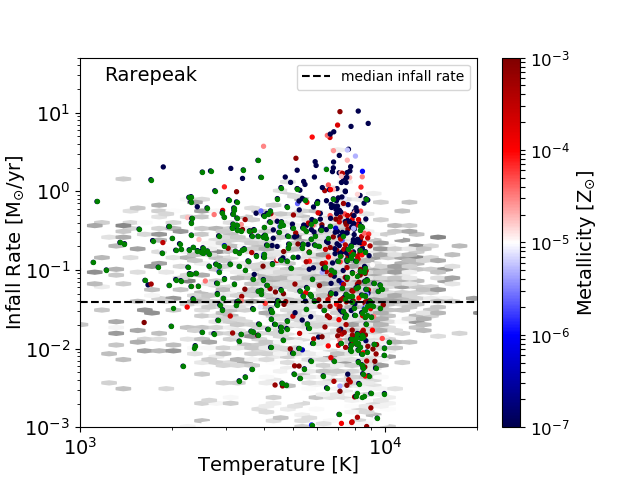
\includegraphics[width=0.525\textwidth]{FIGURES/Rarepeak_MdotTZ.png}
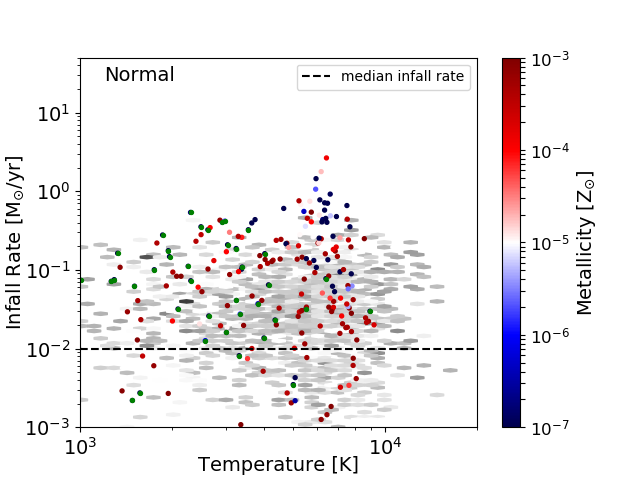
\includegraphics[width=0.525\textwidth]{FIGURES/Normal_MdotTZ.png}}
\caption{\textit{Left Panel}: The mass infall rate inside 10 pc for \textit{all} atomic
  cooling haloes over all redshift outputs for the \rarepeak simulation. The infall rates are plotted
  against the average temperature of the gas within 10 pc, colour coded by metallicity. Hexbins, in
  grayscale, are used to represent the metal enriched haloes ($Z > 10^{-3}$ \zsolarc). Darker colours
  signify higher metallicity. Blue, red and green circles then represent the lower metallicity
  haloes. Red circles represent haloes metallicities with $10^{-3} $ \zsolar $\gtrsim
  Z \gtrsim 10^{-5}$ \zsolarc while blue circles represent metal-poor or metal-free
   haloes with $Z \lesssim 10^{-5}$ \zsolarc. Green circles represent haloes which are both
   completely metal-free and star-free. The median infall rate for all of the haloes is marked
   by the dashed black line. \textit{Right Panel}: The same plot for the \normal simulation with
   the exception that the infall rate and temperatures are calculated within 50 pc of the centre.
   The \normal simulation has less high ($ \gtrsim 1 $ \msolaryrc) infall haloes and also
   significantly less metal-poor haloes.} \label{Fig:Scatter}
\end{center} \end{minipage}

\end{figure*}
%%%%%%%%%%%%%%%%%%%%%%%%%%%%%%%%%%%%%%%%%%%%%%%%%%%%%%%%%%%%%%%%%%%%%%%%%%%%%%%%%%%%%%%%%%%%%%%%%%%%%%%%%
\indent The next heavy seed scenario is arguably the most well studied. In this scenario very high
mass accretion rates onto embryonic proto-stars allows for the creation of super-massive stars (SMSs)
\citep{Shapiro_1979, Begelman_2008, Schleicher_2013, Hosokawa_2013, Inayoshi_2014, Sakurai_2016,
  Umeda_2016, Haemmerle_2017,Woods_2017, Woods_2018, Regan_2018b}. \cite{Sakurai_2016} calculated
that a critical mass accretion rate of 0.04 \msolaryr is required to create a SMS.
Once this level of accretion is maintained the stellar atmosphere can inflate and the star becomes
bloated, causing the surface temperatures to drop to approximately 5000 K \citep{Hosokawa_2013, 
Woods_2017}. \\
\indent In order to achieve the large accretion rates required the general assumption has been
that a metal-free atomic cooling halo is required.
With the mass accretion rate onto a halo scaling as $dM/dt \propto T^{3/2}$ such haloes would appear
to be optimal regions to support high mass infall. The absence of metals removes a cooling pathway for
the gas which would otherwise potentially cause the gas to cool and fragment into smaller, lower
mass, stars thus preventing the formation of a massive central object. A further criteria is that the
atomic cooling halo should have had no previous episode of star formation (which would have
internally enriched the halo with metals). In order to achieve such a pristine halo the \molH content
also must be suppressed. Many studies have investigated pathways to achieve this, the main pathways
investigated have been to employ strong Lyman-Werner (LW) fluxes \citep{Dijkstra_2008, Shang_2010,
  Regan_2014b, Latif_2014b, Agarwal_2015a, Latif_2015, Regan_2016a, Regan_2017, Regan_2018a},
baryonic streaming velocities
\citep{Tseliakhovich_2010, Tanaka_2014, Hirano_2017, Schauer_2017}, collisions of massive
proto-galaxies \citep{Mayer_2010, Mayer_2014, Inayoshi_2015} and finally dynamically heating caused
by a succession of minor and major mergers \citep{Yoshida_2003a, Fernandez_2014, Wise_2019}. \\
\indent The goal of this study is to examine the role that metal-enriched haloes may play in the
  formation of SMSs. 
  To do this we examine the Renaissance datasets and look for haloes that display high mass infall
  rates towards the centre of the halo regardless of the metallicity of the halo. Previously, as
  discussed above, the focus of studies has been on metal-free haloes. What we do here is expand
  the search for supermassive star haloes into the regime of those haloes which were previously
  enriched. The formation of SMSs in metal enriched haloes has recently being investigated by
  \cite{Chon_2020}. They used high-resolution smoothed particle hydrodynamics simulations to
  show that even in cases where the gas metallicity is up to $Z \sim 10^{-3}$ \zsolar that
  SMSs can still form. \cite{Chon_2020} showed that the pathway to formation varies
  somewhat between the purely metal-free case ($Z \lesssim 5 \times 10^{-5}$ \zsolarc) and the
  metal enriched
  case  ($Z \gtrsim 10^{-3}$ \zsolarc) but that the end result remains the same - the formation
  of a massive central object with average accretion rates of approximately 0.1 \msolaryrc.
  Taking these results into account we therefore examine the Renaissance datasets looking
  for the highest infall haloes across all outputs while also examining their metallicities. 

\section{Renaissance Datasets} \label{Sec:RenaissanceDatasets}
The Renaissance Simulations were carried out on the Blue Waters supercomputer facility using the
adaptive mesh refinement code \enzo\citep{Enzo_2014}\footnote{https://enzo-project.org/}. \enzo
has been extensively used to study the formation of structure in the early universe
\citep{Abel_2002, OShea_2005b, Turk_2012, Wise_2012b, Wise_2014, Regan_2015, Regan_2017}. In particular
\enzo includes a ray tracing scheme to follow the propagation of radiation from star formation and
black hole formation \citep{WiseAbel_2011} as well as a detailed multi-species chemistry model that
tracks the formation and evolution of nine species \citep{Anninos_1997, Abel_1997, Grackle}. In
particular the photo-dissociation of \molH is followed, which is a critical ingredient for
determining the formation of the first metal-free stars \citep{Abel_2000}. 

The datasets used in this study were originally derived from a simulation of the universe in a 28.4
\mpch on the side box using the WMAP7 best fit cosmology. Initial conditions were generated using
MUSIC \citep{Hahn_2011} at z = 99. A low resolution simulation was run until z = 6 in order to
identify three different regions for re-simulation \citep{Chen_2014}. The volume was then smoothed
on a physical scale of 5 comoving Mpc, and regions of high
($\langle\delta\rangle \equiv \langle\rho\rangle(\Omega_{\rm M} \rho_{\rm c}) - 1 \simeq 0.68$),
average ($\langle\delta\rangle \sim 0.09)$), and low ($\langle\delta\rangle \simeq -0.26)$)
mean density were chosen for re-simulation. These sub-volumes were then referred to as the
\rarepeak region, the \normal region  and the \void region. The \rarepeak region has a comoving
volume of 133.6 Mpc$^3$, and the \normal and \void regions both have comoving volumes of 220.5
Mpc$^3$. Each region was then re-simulated with an effective initial resolution of $4096^3$ grid
cells and particles within these sub-volumes of the larger initial simulation. This gives a maximum
dark matter particle mass resolution of $2.9 \times 10^4$ \msolarc. For the re-simulations of the
\voidc, \normal and \rarepeak regions further refinement was allowed throughout the sub-volumes up
to a maximum refinement level of 12, which corresponded to 19 pc comoving spatial resolution. Given
that the regions focus on different over-densities each region was evolved forward in time to
different epochs. The \rarepeak region, being the most over-dense and hence the most
computationally demanding at earlier times, was run until z = 15. The \normal region ran until z =
11.6, and the \void region ran until z = 8. In all of the regions the halo mass function was very
well resolved down to M$_{\rm halo} \sim 2 \times 10^6$ \msolarc. The \rarepeak regions contained
822 galaxies with masses larger than $10^9$ \msolar at z = 15, the \normal region contained 758
such galaxies at z = 11.6, while the \void region contained 458 such galaxies at z = 8.
In this study we examine only the \rarepeak and \normal regions.
%%%%%%%%%%%%%%%%%%%%%%%%%%%%%%%%%%%%%FIGURE 2 (Hexbins)%%%%%%%%%%%%%%%%%%%%%%%%%%%%%%%%%%%%%%%%%%%%%%%%%%%%%%%%%%%
\begin{figure*}
\centering
\begin{minipage}{175mm}      \begin{center} 
\centerline{
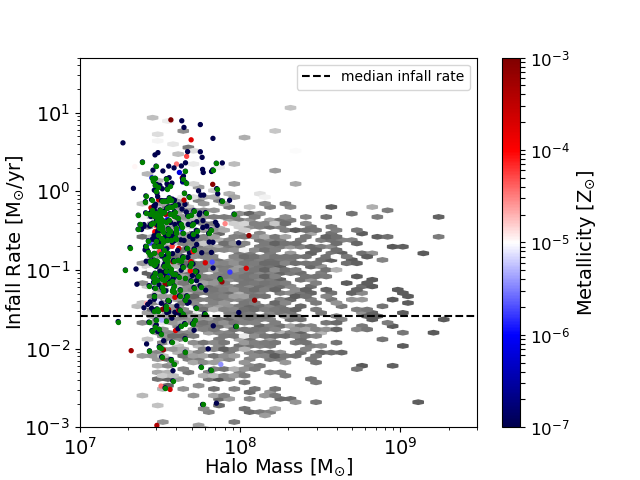
\includegraphics[width=0.525\textwidth]{FIGURES/Rarepeak_MdotMHaloZ_Hexbin.png}
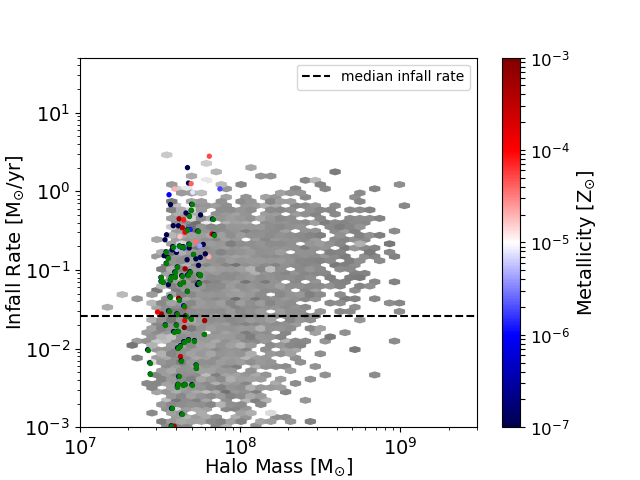
\includegraphics[width=0.525\textwidth]{FIGURES/Normal_MdotMHaloZ_Hexbin.png}}
\caption{\textit{Left Panel}: The mass infall rate inside 10 pc for \textit{all} atomic
  cooling haloes over all redshift outputs for the \rarepeak simulation. The infall rates
  are plotted against the mass of the halo in which the infall rate is
  calculated. The haloes are further sub-divided into the most metal enriched haloes
  i.e. those with solar metallicities greater than 10$^{-3}$ \zsolar and shown in grayscale with
  hexbins. Darker hexbins represent higher metalicities. Metal poor haloes are then represented
  by circles in an overplotted scatter plot. The metal-poor haloes, those with metallicities
  $Z < 10^{-3}$ \zsolar populate the halo mass range just below $10^{8}$ \msolar predominantly.
  Green cicles represent those haloes that are both metal-free and star-free. 
  \textit{Right Panel}: The same plot for the \normal simulation with the exception that the infall
  rates are again calculated within 50 pc of the centre. By again sub-dividing the haloes we see
  that the \normal region has significantly fewer metal-poor haloes in this halo mass range.
  Virtually all of the haloes in the \normal region are already metal enriched and certainly the
  highest mass infall haloes, in the \normal region, are metal enriched. 
  The median infall rate for all of the haloes is marked by the dashed black line in both panels.}
\label{Fig:HaloMass}
\end{center} \end{minipage}

\end{figure*}
%%%%%%%%%%%%%%%%%%%%%%%%%%%%%%%%%%%%%%%%%%%%%%%%%%%%%%%%%%%%%%%%%%%%%%%%%%%%%%%%%%%%%%%%%%%%%%%%%%%%%%%%%
%%%%%%%%%%%%%%%%%%%%%%%%%%%%%%%%%%%%%FIGURE 3 (Hexbins)%%%%%%%%%%%%%%%%%%%%%%%%%%%%%%%%%%%%%%%%%%%%%%%%%%%%%%%%%%%
\begin{figure*}
\centering
\begin{minipage}{175mm}      \begin{center} 
\centerline{
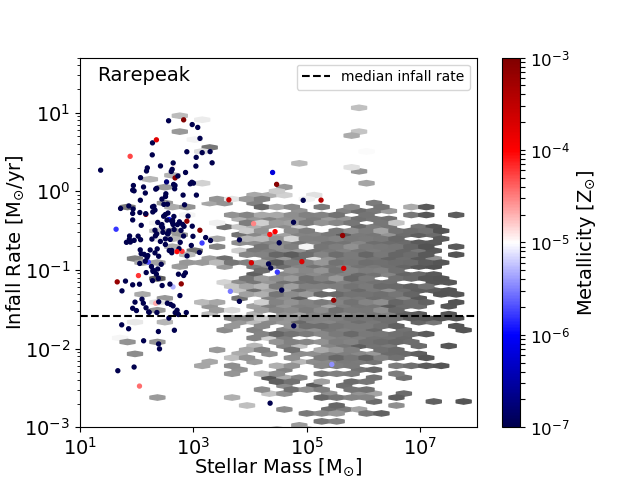
\includegraphics[width=0.525\textwidth]{FIGURES/Rarepeak_MdotMstellarZ_Hexbin.png}
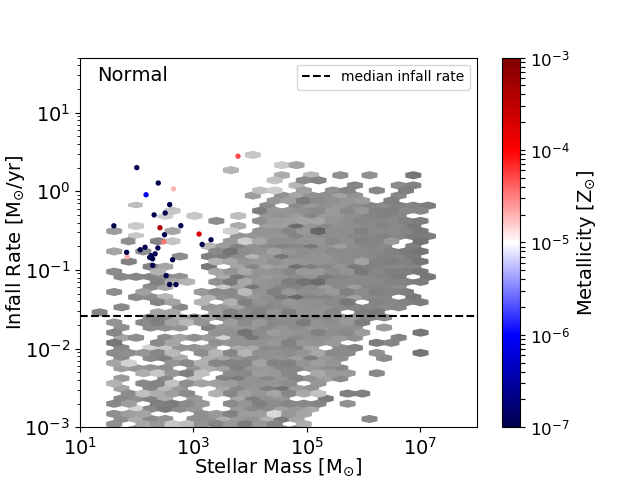
\includegraphics[width=0.525\textwidth]{FIGURES/Normal_MdotMstellarZ_Hexbin.png}}
\caption{\textit{Left Panel}: The mass infall rate inside 10 pc for \textit{all} atomic
  cooling haloes over all redshift outputs for the \rarepeak simulation. In this case,
  the infall rates are plotted against the stellar mass of the halo in which the infall rate is
  calculated. The haloes are further sub-divided into the most metal enriched haloes
  i.e. those with solar metallicities greater than 10$^{-3}$ \zsolar and shown in grayscale with hexbins.
  Darker hexbins represent higher metallicities. Metal poor haloes are then represented by circles in
  an overplotted scatter plot. As can be seen from the left panel there are a large fraction of
  metal poor halo residing in low stellar mass haloes. A substantial fraction of these haloes have
  high infall rates. 
  \textit{Right Panel}: The same plot for the \normal simulation with the exception that the infall rates are 
  again calculated within 50 pc of the centre. By again sub-dividing the haloes we see that the \normal
  region has significantly fewer metal-poor haloes in this stellar mass range. Virtually all of the
  haloes in the \normal region are already metal enriched and certainly all of the high infall haloes,
  in the \normal region, are metal enriched. 
  The median infall rate for all of the haloes is marked by the dashed black line in both panels.} \label{Fig:StellarMass}
\end{center} \end{minipage}

\end{figure*}
%%%%%%%%%%%%%%%%%%%%%%%%%%%%%%%%%%%%%%%%%%%%%%%%%%%%%%%%%%%%%%%%%%%%%%%%%%%%%%%%%%%%%%%%%%%%%%%%%%%%%%%%%
%%%%%%%%%%%%%%%%%%%%%%%%%%%%%%%%%%%%%FIGURE 4 (Histogram)%%%%%%%%%%%%%%%%%%%%%%%%%%%%%%%%%%%%%%%%%%%%%%%%%%%%%%%%%%%
\begin{figure*}
\centering
\begin{minipage}{175mm}      \begin{center} 
\centerline{
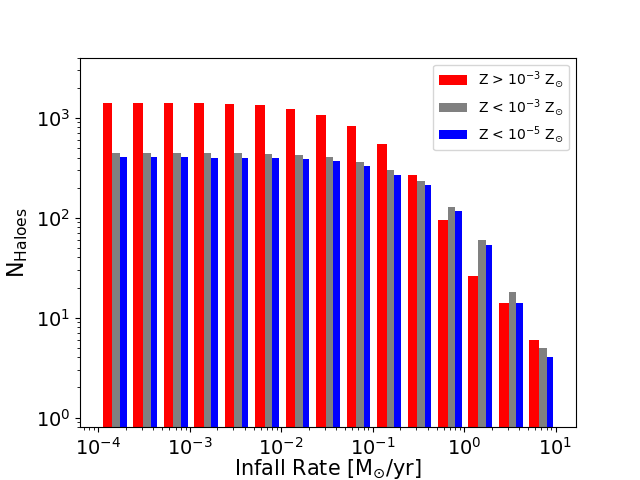
\includegraphics[width=0.525\textwidth]{FIGURES/Rarepeak_NHaloes.png}
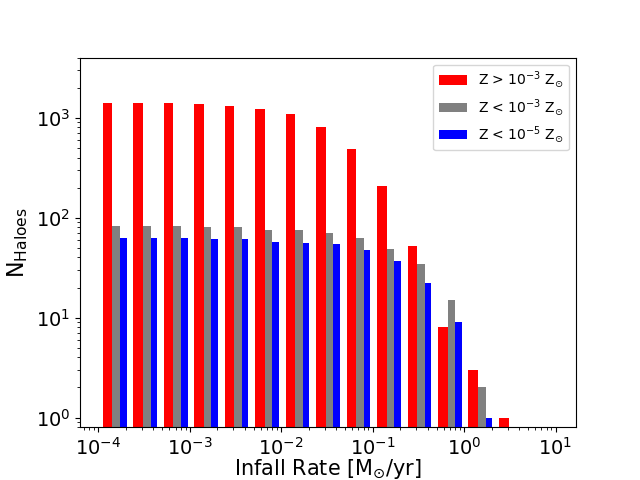
\includegraphics[width=0.525\textwidth]{FIGURES/Normal_NHaloes.png}}
\caption{\textit{Left Panel}: The cumulative number of haloes with infall rates greater than the given
  x-axis value for the \rarepeak region.  The total number of \rarepeak haloes across all outputs
  is 2175. Infall rates are again calculated at 10 pc from the halo centre.
  Haloes are sub-divided into haloes with metallicities Z $< 10^{-1}$ \zsolar (red bars),
  Z $< 10^{-3}$ \zsolar (grey bars) and  Z $< 10^{-5}$ \zsolar (blue bars). In the \rarepeak region
  the number of haloes with high infall rates (right-hand bars in panel) and low to moderate metallicities
  (i.e. Z$ < 10^{-3}$ \zsolarc) is a significant fraction of the total number of haloes. Nonetheless there
  are also metal enriched haloes with very high infall rates. \textit{Right Panel}: The distribution of
  infall rates for the \normal region. The  total number of \normal haloes across all outputs is 2432.
  In the \normal region the number (or equivalently fraction) of metal-poor haloes is significantly reduced
  compared to the \rarepeak region. We also again see that there are fewer haloes with infall rates greater
  than 1 \msolaryrc. } \label{Fig:Histogram}
\end{center} \end{minipage}

\end{figure*}
%%%%%%%%%%%%%%%%%%%%%%%%%%%%%%%%%%%%%%%%%%%%%%%%%%%%%%%%%%%%%%%%%%%%%%%%%%%%%%%%%%%%%%%%%%%%%%%%%%%%%%%%%

\subsection{Results} \label{Sec:Results}

As discussed in \S \ref{Sec:RenaissanceDatasets} the \rarepeak dataset represents an overdense
region of the Universe with a large selection of galaxies while the \normal region represents a
region with an average density comparable to the cosmic mean. We begin our analysis of those two
datasets by examining only those galaxies which lie inside the high resolution region and which
have masses greater than the atomic cooling limit. In this work we define the atomic cooling
limit as
\begin{equation}
M_{\rm atm} = 10^8 \times \Big ({ {1 + z} \over {10}} \Big )^{-1.5} M_{\odot}
\end{equation}
where M$_{\rm atm}$ is the atomic cooling limit mass and $z$ is the redshift.
For both datasets, we then filter each halo based on the mass infall rate onto that halo.
We calculate the instantaneous mass infall rate using the standard continuity equation:
\begin{equation}  
  \dot{M} = 4 \pi R^2 \rho(R) V_{\rm rad}(R)
\end{equation}
where  $\dot{M}$ is the mass infall rate, R is the radius at which the infall rate is calculated,
$\rho(R)$ is the gas density at that radius and $V_{\rm rad}(R)$ is the radial velocity at that radius.
For the \rarepeak region the mass infall rate is calculated as the median infall rate within 10 pc
of the centre of the halo. For the \normal region  the mass infall rate was calculated as the median
infall rate within 50 pc of the centre of the halo. The reason for the difference was
that the \normal region shows more disruption to haloes, on average, in the centre and so in
order to get an accurate picture of mass infall rates for the \normal haloes a larger radius
was required. \\
\indent The \rarepeak simulation was run until a redshift of 15 but we
examine all of the outputs\footnote{There are 40 \rarepeak outputs between $z = 24$ and $z = 15$.}
from the dataset. For the \normal datasets we adopt the exact same procedure except that
the \normal simulation runs until z = 11.6 and again we examine all of the
outputs\footnote{There are 70 \normal outputs between $z = 24$ and $z = 15$.}.\\
\indent For the \rarepeak haloes at the final output time ($z = 15$) we find that there are
50 haloes with mass infall rates greater than 1 \msolaryr while in the \normal region at its final
output time ($z = 11.6$) we find that there are 20 haloes with mass infall rates
greater than 1 \msolaryrc. However, to be more comprehensive we examine all 110 outputs available to
us across both the \rarepeak and \normal regions and examine the infall rate in each of the haloes,
with masses greater than the atomic cooling limit, in each output. \\
%%%%%%%%%%%%%%%%%%%%%%%%%%%%%%%%%%%%%FIGURE 5%%%%%%%%%%%%%%%%%%%%%%%%%%%%%%%%%%%%%%%%%%%%%%%%%%%%%%%%%%%
\begin{figure*}
\centering
\begin{minipage}{175mm}      \begin{center} 
\centerline{
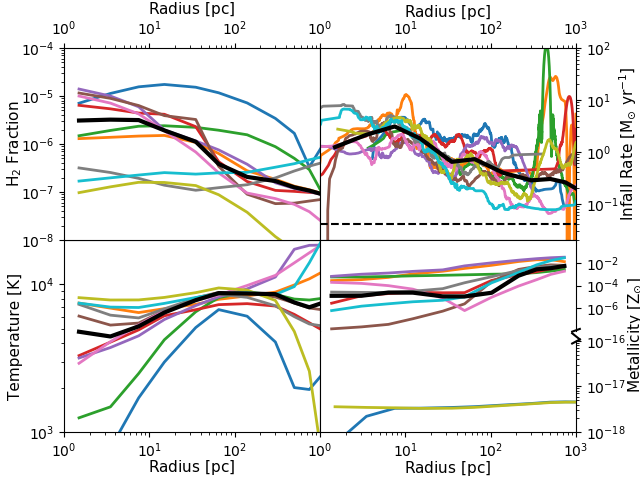
\includegraphics[width=0.525\textwidth]{FIGURES/MultiPlot_Rarepeak.png}
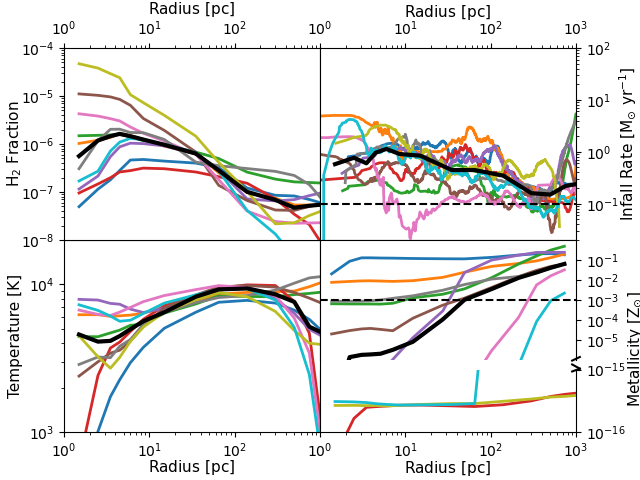
\includegraphics[width=0.525\textwidth]{FIGURES/MultiPlot_Normal.png}}
\caption{\textit{Left Panel}: Radial profiles for the top 10 highest infall rate haloes. For
  each halo the temperature, \molH fraction, infall rate and metallicity are given for
  each halo. The median radial values for each quantity are shown using the
  thick black line in each panel. The metallicity (bottom right panel) of haloes can span many
  orders of magnitude and so that panel is artificially cut in the middle. Nonetheless, what is
  clear is that the majority of high infall rate haloes are metal enriched with only a single
  metal halo in the top 10 highest accretors. \textit{Right Panel}: The same plot for the \normal
  haloes. The features are broadly similar with the exception that no truely metalfree haloes are
  among the highest accretors in the \normal region and also that the infall rates for the \rarepeak
  haloes are higher than those of the \normal haloes. 
} \label{Fig:RadialProfiles}
\end{center} \end{minipage}

\end{figure*}
%%%%%%%%%%%%%%%%%%%%%%%%%%%%%%%%%%%%%%%%%%%%%%%%%%%%%%%%%%%%%%%%%%%%%%%%%%%%%%%%%%%%%%%%%%%%%%%%%%%%%%%%%
\subsection{Central mass infall rates}
\indent We first plot the mass infall rate of each halo against three different halo
characteristics. First in Figure \ref{Fig:Scatter} we show a scatter plot of the mass infall rates
against the inner halo temperature. Secondly in Figure \ref{Fig:HaloMass} we plot the halo infall
rate against the total halo mass, and finally in Figure  \ref{Fig:StellarMass} we show the halo
infall rate against the stellar mass of each halo. We begin by analysing Figure \ref{Fig:Scatter}. \\
\indent In the left panel of Figure \ref{Fig:Scatter} we show the results from the \rarepeak
simulation and in the right panel the results from the \normal simulation. Each point shows the mass
infall rate averaged over 10 pc for the \rarepeak region (50 pc
for the \normal region). The mass infall rates are plotted against the average temperature within
the same region in each halo. There are two colour codes on the plot. The grayscale
hexbins capture all metallicities\footnote{Note that all metallicities
  referred to in this paper are gas phase metallicities.}
greater than $Z = 10^{-3}$ \zsolarc. Each coloured circle then refers to
the metallicities of the metal-poor and metal-free haloes. Red circles indicate
mildly metal enriched regions ( $10^{-5} \lesssim Z/Z_\odot \lesssim 10^{-3}$ )  while blue circles indicate
metal poor regions  ( $Z \lesssim 10^{-5}$ \zsolar ) . We also include green circles
on the plot to indicate haloes which are completely metal-free and star-free. \\
\indent Some results are immediately clear from a comparison of the panels in Figure
\ref{Fig:Scatter}. The \rarepeak region clearly has significantly more haloes that have lower
metallicities and it also has more haloes
with high infall haloes. Nonetheless, while there are a number of high mass infall,
metal-poor haloes, in the \rarepeak region - the highest mass infall halo is infact metal enriched
and there are comparable numbers of high infall haloes which are both metal enriched and metal-poor.
The metal-free and star-free haloes (green circles) show a strong scatter and are not preferentially
high accretors. The metal-free and star-free haloes do populate the lower temperature parts of the
phase space however and this is because they have no ongoing star formation (by definition) and so
the temperature of the gas is determined purely by the competition between gas cooling and
dynamical and compressional heating. The other metal-poor haloes, especially those with temperatures
close to T = $10^4$ K are likely being heated by ongoing star formation with atomic line
cooling keeping the temperature close to T = $10^4$ K. 
The haloes in the \normal region are in general much more metal enriched. Infact of
all of the haloes plotted only 9 haloes have metallicites below  $Z = 10^{-3}$ \zsolarc. The
prevalence of metal enrichment is clearly much stronger in the \normal region.\\
\indent In Figure \ref{Fig:HaloMass} we plot the mass infall rate against the total (dark matter
+ gas) halo mass. In this representation the metal-poor haloes are strongly clustered, in both
the \rarepeak and \normal regions, at the atomic cooling limit (M$_{\rm atm} \sim 4 \times 10^7$
\msolar). This result is not surprising - once the atomic cooling limit is reached star formation
will begin (if it hasn't already) and from that point onwards it is only a matter of time before
the halo becomes strongly metal enriched. Complementary to this is Figure \ref{Fig:StellarMass}
where we plot the mass infall rate against the stellar mass. In the left panel of Figure
\ref{Fig:StellarMass} we show the scatter/hexbin plot, coloured by metallicity, of the
\rarepeak region. There is a large cluster of haloes, with $Z \lesssim 10^{-3}$ \zsolarc,
with stellar masses of M$_{*} \lesssim 10^3$ \msolarc. These are haloes
populated with PopIII stars and the majority are metal-poor ($Z \lesssim 10^{-5}$ \zsolarc). It should also be
noted that this group of haloes also contain some of the highest mass infall rates. The \normal
region contains significantly fewer haloes with metallicities, $Z \lesssim 10^{-3}$ \zsolarc. Similarly, to the
\rarepeak region, the majority (all in this low numbers case) have stellar masses with
M$_{*} \lesssim 10^3$ \msolarc. The haloes in the \normal region are also more metal enriched compared
to the \rarepeak region and this can be seen by the darker grayscale hexbins in the \normal region.
From Figures \ref{Fig:Scatter}, \ref{Fig:HaloMass} and \ref{Fig:StellarMass} we see that there exists
a sizeable minority of high mass infall haloes with low metallicity ($Z \lesssim 10^{-5}$ \zsolarc). These
haloes, due to their large mass infall rates, makes them strong candidates for super-massive
star formation \citep{Woods_2018, Chon_2020}. However, equally there exists a large population of
high mass-infall, metal enriched, haloes. Some of these haloes could potentially support SMS formation
if the metal mixing within the halo is inhomogeneous. We will discuss this point further in \S
\ref{Sec:Discussion}. First we quantify the relative ratios of metal-enriched
and metal poor haloes in Figure \ref{Fig:Histogram}.
%%%%%%%%%%%%%%%%%%%%%%%%%%%%%%%%%%%%%FIGURE 6%%%%%%%%%%%%%%%%%%%%%%%%%%%%%%%%%%%%%%%%%%%%%%%%%%%%%%%%%%%
\begin{figure*} 
\centering
\begin{minipage}{175mm}      \begin{center} 
\centerline{
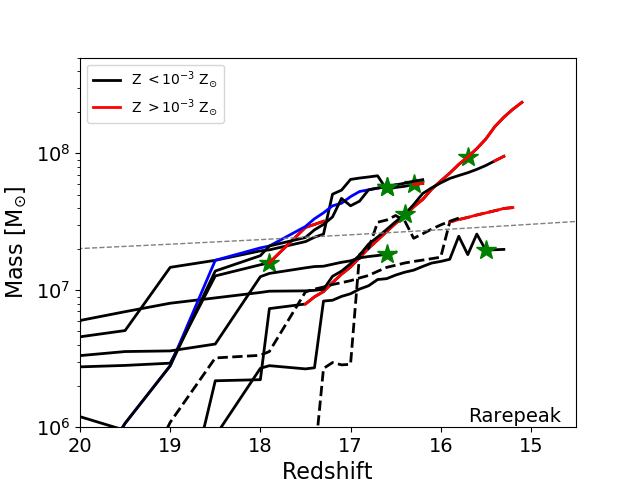
\includegraphics[width=0.525\textwidth]{FIGURES/Rarepeak_MassRedshift.png}
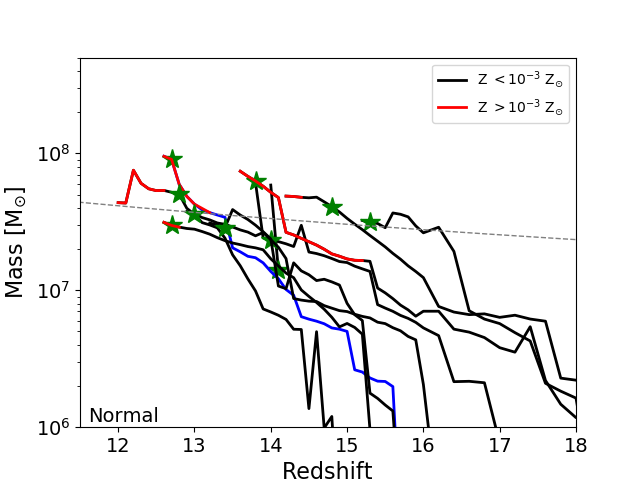
\includegraphics[width=0.525\textwidth]{FIGURES/Normal_MassRedshift.png}}
\caption{\textit{Left Panel}: The growth rate as a function of redshift for the \rarepeak haloes identified in the left
  panel of Figure \ref{Fig:RadialProfiles}. Metal poor ($Z < 10^{-6}$ \zsolarc) haloes are marked in black while
  metal enriched haloes ($Z > 10^{-6}$ \zsolarc) are marked in red. Note that a halo can become metal enriched
  during it's evolution. The enrichment can come from internal or external sources. Green stars indicate the
  redshift at which star formation first occurs in each halo. Two haloes have remained star free until their
  detection as high infall haloes (dashed lines). The dashed blue line in each panel is the atomic cooling limit.
  \textit{Right Panel}: The same mass growth plot for the \normal region. The \normal region contains at its final
  output time contains less metal-poor haloes that the \rarepeak region (see also Figure \ref{Fig:Scatter}) and
  hence the fraction of metal enriched (red) lines is higher. Nonetheless, a metal-free star-free halo which
  is rapidly accreting still exists. 
}\label{Fig:GrowthRates}
\end{center} \end{minipage}

\end{figure*}
%%%%%%%%%%%%%%%%%%%%%%%%%%%%%%%%%%%%%%%%%%%%%%%%%%%%%%%%%%%%%%%%%%%%%%%%%%%%%%%%%%%%%%%%%%%%%%%%%%%%%%%%%
\subsection{Halo Ratios}
In Figure \ref{Fig:Histogram} we show the cumulative number of haloes with infall rates greater than
the given value on the x-axis. The x-axis runs from $\dot{M}(R) = 10^{-4}$ \msolaryr to 
$\dot{M}(R) = 10^{1}$ \msolaryrc. As the plot runs from left to right the number of haloes with a
mass infall rate greater than a given value diminishes as expected. The mass infall rate,
$\dot{M}(R)$, is calculated as the average value within 10 pc of the centre for the \rarepeak region
and within 50 pc of the centre for the \normal region. In Figure  \ref{Fig:Histogram} the
\rarepeak region is shown in the left panel while the \normal region is shown in the right hand
panel. Bars in each panel are coloured as follows: red bars are for haloes with metallicities
($Z > 10^{-3}$ \zsolarc), grey bars are for haloes with ($Z < 10^{-3}$ \zsolarc) and blue bars are for
haloes with ($Z < 10^{-5}$ \zsolarc). In total there are 2175 haloes found across all outputs in
the \rarepeak region and 2432 haloes found across all outputs in the \normal region. \\
\indent Concentrating first on the \rarepeak region we see that there are a small number of
haloes ($\sim 35$) with mass infall rates greater than 1 \msolaryrc. These haloes are almost
completely evenly spread across metal-enriched ($Z > 10^{-3}$ \zsolarc) and
slightly metal-enriched/metal-poor haloes ($Z < 10^{-3}$ \zsolarc). Haloes with between
($10^{-3}$ \zsolar $> Z > 10^{-5}$ \zsolarc) only add slightly (i.e. difference in height between the
blue and grey bars) to the total number of haloes that
have been shown to result in SMS formation \citep{Chon_2020}. As we move along the histogram to the
left and concentrate on haloes with mass infall rates greater than 0.1 \msolaryr we see the
number of metal enriched haloes grow compared to
metal-poor haloes. If we allow all haloes (independent of metallicity) with mass infall rates greater
than  0.1 \msolaryr to be super-massive star candidates then the number of candidate haloes can
increase by at least an order of magnitude compared to even the slight metal-enriched case. We will
come back to this point in \S \ref{Sec:Discussion}. \\
\indent In the right hand panel of Figure \ref{Fig:Histogram}
we show the same histogram for the \normal region. In this case there is dearth of metal-poor haloes
with mass infall rates of greater than 1 \msolaryr - although there are a comparable number of
metal-enriched haloes compared to the \rarepeak region for the same mass infall rates. In the
\normal region the haloes are dominated by metal-enriched haloes with only a small number (8)
of haloes with low metallicity. On the face of it this suggests that the \normal region will
support only a small number of super-massive star candidates. However, similar to the \rarepeak
if we relax the criteria for super-massive star formation and consider also metal-enriched haloes
then the number of possible candidate haloes can increase by a factor of over a 100 in the \normal
region when considering haloes with mass infall rates, $\dot{M} > 0.1 $ \msolaryrc. 



\subsection{The Highest Accretors}
\indent We next assess the ten highest accreting haloes in each region. In Figure
\ref{Fig:RadialProfiles} we plot the radial profiles of each of the highest accreting haloes.
%Haloes are excluded from the plot if they have undergone a recent supernovae explosion (and have
%temperatures in excess of $10^5$ K within their virial radius). Such haloes can lead to spurious
%mass infall rates.
In each figure we show the temperature, \molH fraction, mass infall rates and
metallicity of each halo as a function of radius. The thick black line in each panel gives the
median value for the given quantity. Values across the two panels are broadly similar. The
metallicities of the \rarepeak haloes (left panel) cover a larger range with two of the highest
accreting haloes remaining metal free. Note that the metallicity sub-panel of the \rarepeak panel
is split between metal-enriched and metal-free haloes. Mass infall rates in both the \rarepeak
and \normal regions, for these select haloes, are comfortably above the critical value thought to
be necessary for SMS formation (0.04
\msolaryr \citep{Sakurai_2016}) even though some of the haloes have metallicity values of $Z > 10^{-3}$
\zsolar which may lead to the formation of lower mass stars compared to lower metallicities
\citep{Chon_2020}. This critical value for the mass infall rate is plotted as the dashed black line in
the top right hand sub-panel of each panel. While mass infall rates determined at this radius is no
way a guarantee that this will lead to similar accretion rates onto a protostar, the high rates do
suggest that large amounts of matter are being transferred to the halo centre at least. \\
\indent In Figure \ref{Fig:GrowthRates} we plot the halo mass history of the high infall
rate haloes shown in Figure \ref{Fig:RadialProfiles} with the \rarepeak and \normal haloes
shown on left- and right-hand panels, respectively. 
Metal poor haloes are defined as those with gas phase metallicities less than
$10^{-5}$ \zsolarc. Metal poor haloes are coloured in black while metal enriched haloes are coloured
red. Haloes can become metal enriched either through internal star formation and supernovae or
alternatively can become metal enriched through external enrichement processes
\citep[e.g.][]{Smith_2015}. Where star formation first
occurs in a halo the redshift of star formation is denoted by a green star on the halo growth line. 
Haloes which remain completely star free are marked as dashed lines. \\
\indent In the \rarepeak region there are two
star-free haloes. One remains star free and metal poor all the way to z = 15 (the final output time).
The other becomes externally metal enriched at $z \sim 17.2$ but fails to form any stars up until 15.2
(where it was detected as a high infall halo). The metal mixing within the other eight haloes is far
more varied. Some haloes are externally enriched and then proceed to form stars later in their
evolution while others form stars and then become internally enrich themselves. 
However, given that these are relatively massive galaxies with deep potential wells
the metal mixing can be gradual in some haloes but more rapid in others. The varying efficiency of
metal mixing means that some haloes, with prior star formation, are nonetheless suitable candidates
for supermassive star formation when mixing is inefficient but high accretion rates prevail. \\
\indent In the \normal region haloes are, as we have seen previously, much more likely to be
metal enriched. This is reflected in the growth plots. Most of the haloes become metal enriched
although one halo does remain metal poor ($Z < 10^{-5}$ \zsolarc) and star-free as shown by the dashed
line. Furthermore, several of these high accreting haloes formed their stars earlier in their merger
history often due to external metal enrichement. We now explore the implictaions of these results for
the formation of super-massive stars. 

\section{Discussion and Conclusions} \label{Sec:Discussion}
The goal of this paper is to examine the prevalence of high infall rate halos in the
Renaissance Simulations which in turn are thought to represent very accurately the
behaviour of structure formation in our Universe \citep{Chen_2014, Xu_2013, Xu_2014, OShea_2015,
  Barrow_2017, Wise_2019}. A high mass accretion rate onto an embryonic proto-star is the
single most important criteria for the formation of a SMS \citep{Hosokawa_2013, Sakurai_2016,
  Woods_2018}. Therefore, we examine the Renaissance datasets for haloes which are experiencing
rapid gas inflow in their centres. While, rapid gas inflow to the halo centre does not guarantee
that a SMS will ultimately form it is however very likely to be a necessary condition. \\
\indent Previous investigations of SMS candidate haloes have almost universally focused on
metal-free haloes in which the equation of state of the gas was determined by the gas phase
cooling mechanisms of hydrogen and helium. Here, we extend the analysis to haloes that are both
metal-poor and metal-enriched. If the number of haloes that support SMS formation can be extended to
include also these haloes which are metal enriched (at least perhaps up to some metallicity or
due to metal enrichment inhomogeneity) then the
number density of candidate direct collapse black hole seeds will increase accordingly and so is of
immense interest to the community. Previous direct collapse black hole number densities have
tended to show that when including metal-free haloes only  that the number of direct collapse
black holes may be either insufficient or just sufficient to explain the number of density of
high-z quasars \citep{Agarwal_2012, Visbal_2014b, Agarwal_2015b, Latif_2014a,
  Valiante_2016, Habouzit_2016, Valiante_2017, Habouzit_2017, Regan_2017}. \\
%%%%%%%%%%%%%%%%%%%%%%%%%%%%%%%%%%%%%FIGURE 7%%%%%%%%%%%%%%%%%%%%%%%%%%%%%%%%%%%%%%%%%%%%%%%%%%%%%%%%%%%
\begin{figure}
   \centering 
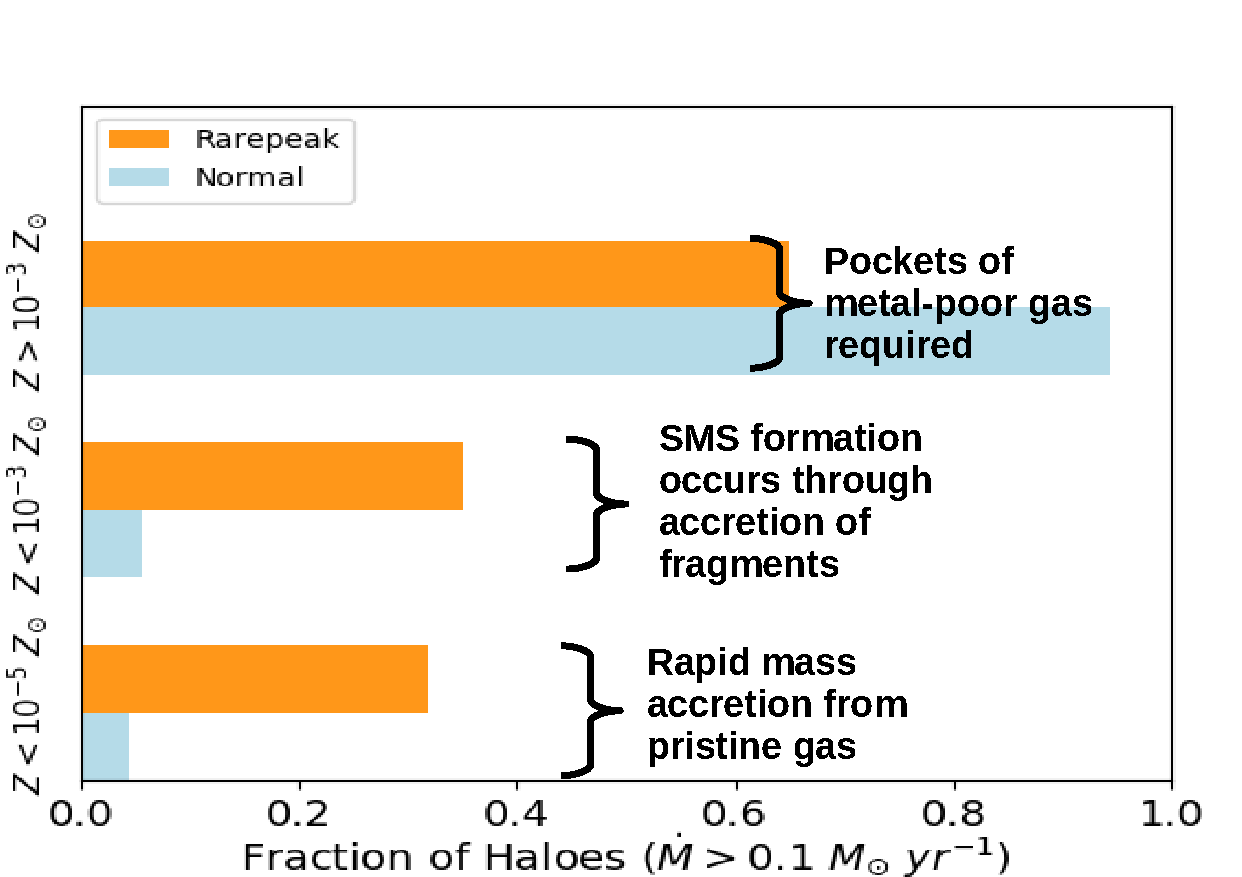
\includegraphics[width=0.525\textwidth]{FIGURES/FinalPlot-crop.pdf}
\caption{The fraction of haloes which have metallicities of $Z > 10^{-3}$ \zsolar,
  $Z < 10^{-3}$ \zsolar and $ Z < 10^{-5}$ \zsolar and have mass infall rates greater than
  0.1 \msolaryrc. The vast majority of haloes ($\sim 93$\%) are metal enriched and hence within
  those haloes pockets of metal-poor gas will be required for SMS to occur. As the metallicity
  decreases the ability of haloes to form SMS for a given accretion rate increases. The fraction of
  metal enriched haloes also decreases with accretion rate (see Figure \ref{Fig:Histogram}).} \label{Fig:Fractions}
\end{figure}
%%%%%%%%%%%%%%%%%%%%%%%%%%%%%%%%%%%%%%%%%%%%%%%%%%%%%%%%%%%%%%%%%%%%%%%%%%%%%%%%%%%%%%%%%%%%%%%%%%%%%%%%%
\indent \cite{Chon_2020} have recently shown, through dedicated high resolution numerical simulations
of the collapse of candidate SMS haloes that metallicities up to $Z \lesssim 10^{-3}$ \zsolar
are compatible with SMS formation. They showed that for metallicities of $Z \lesssim 5 \times 10^{-5}$ \zsolar
that the behaviour of SMS formation is the same as the metal-free case i.e. SMS formation results
directly from the rapid accretion of pristine gas. \cite{Tagawa_2020} came to similar conclusions
using a semi-analytic approach. \cite{Chon_2020} further showed that when the metallicity
reaches intermediate values, $5 \times 10^{-5}$ \zsolar $ < Z < 10^{-3}$ \zsolarc, then while
the gas does fragment, the fragments nonetheless coalesce onto the growing protostar and the
result is a SMS. In the case of high metal enrichement,  $Z \gtrsim 10^{-3}$ \zsolar
they find that the gas cooling becomes too rapid and that the gas fragments into low mass fragments
and SMS formation is inhibited. However, there remains the possibility that even in these
metal-enriched haloes that pockets of metal-poor gas will remain in which SMS formation can occur.
Investigation of this scenario was outside the scope of the \cite{Chon_2020} investigations but given
that metal-mixing has previously being shown to be inefficient \citep[e.g.][]{Smith_2015} this
(metal-enriched) scenario warrants further research. \\
\indent With this in mind we included all high mass infall haloes in our analysis regardless of
metallicity. To do this we examined the Renaissance datasets, analysing
both the \normal and \rarepeak regions. We analysed the simulation volumes and filtered atomic
cooling haloes by their instantaneous mass infall rates in the centre of each halo, at 50 pc for
the \normal haloes and at 10 pc for the \rarepeak haloes.  \\
\indent We found that, as expected, there is a large number of haloes with very high accretion rates
in the centre (see Figure \ref{Fig:Histogram}). At accretion rates
greater than 1.0 \msolaryr there are similar numbers of metal-poor and metal-enriched haloes
(38\%:62\%) in the \rarepeak simulation. In the \normal region the metal-enriched haloes always
outnumber the metal-poor haloes. Relaxing the mass infall criteria to 0.1  \msolaryr we find
that of these ``high-accreting'' haloes a majority of these haloes are either strongly
metal-enriched ($Z > 10^{-3}$ \zsolarc) or mildly metal-enriched
($10^{-5}$ \zsolar $ < Z < 10^{-3}$ \zsolarc). In Figure \ref{Fig:Fractions}  we show the fraction
of high accretion rate ($\dot{M} > 0.1$ \msolaryrc) haloes and their (gas phase) metallicities
for haloes from both the \normal and \rarepeak regions.
The vast majority, 93\%, of highly accreting haloes ($\dot{M} > 0.1$ \msolaryrc) are metal
enriched. In the optimistic case where all of these haloes support SMS formation the boost to
candidate haloes for SMS formation, compared to the metal-poor case, is at least one order of
magnitude. While,
some of these haloes may ultimately be shown through high resolution simulation to not support SMS
formation their high mass infall rates will at a minimum transfer a large baryon content towards the
halo centre which may impact the initial mass function and is worth further investigation.
Below a level of $Z \sim 10^{-3}$ \zsolar the formation of a SMS depends only on the mass infall
rate onto the protostar but those haloes are in the minority being at best 10\% of the total
high accreting halo fraction. \\
\indent Additional high resolution hydrodynamic simulations will be required to
determine the fraction of metal-enriched haloes which can support SMS formation and in particular
whether pockets of metal-poor gas in these haloes can support SMS formation. Clearly, if metals
  become mixed efficiently then these haloes are unsuitable as candidates for SMS formation (we see
no observational evidence of SMS formation in present day low metallicity galaxies). However,
the galaxies studied here are embryonic and have had very few dynamical times in which the
gas mixing can take place and hence metal-poor pockets are much more likely. The addition of (some)
metal-enriched haloes to the number density of direct collapse black hole candidate haloes
would help relieve the current tensions that exist in understanding the formation pathways for
high-z quasars. 

%====================================================================
\section*{Acknowledgments}
%====================================================================

JHW is supported by National Science Foundation grants AST-1614333 and
OAC-1835213, and NASA grant NNX17AG23G.  The simulation was performed on Blue
Waters operated by the National Center for Supercomputing Applications (NCSA)
with PRAC allocation support by the NSF (awards ACI-1514580 and OAC-1810584).
This research is part of the Blue Waters sustained-petascale computing project, which
is supported by the NSF (awards OCI-0725070, ACI-1238993) and the state of
Illinois. Blue Waters is a joint effort of the University of Illinois at
Urbana-Champaign and its NCSA.  The freely available plotting library {\sc
matplotlib} \citep{matplotlib} was used to construct numerous plots within this
paper. Computations and analysis described in this work were performed using the
publicly-available \enzo and \yt{} \citep{YT} codes, which is the product of a
collaborative effort of many independent scientists from numerous institutions
around the world.

%\ref{lastpage}
\bibliographystyle{mn2e_w}
\bibliography{./mybib}
\end{document}
